%!TEX root = /Users/rafaeldurelli/Dropbox/Artigos Elaborados/KDM propagation_2015/sbes_2015_kdm_propagation/sbes2015_kdm_propagation.tex
\section{Motivation and running example} % (fold)
\label{sec:motivation_and_running_example}

\begin{figure*}
	\centering
	% Requires \usepackage{graphicx}
	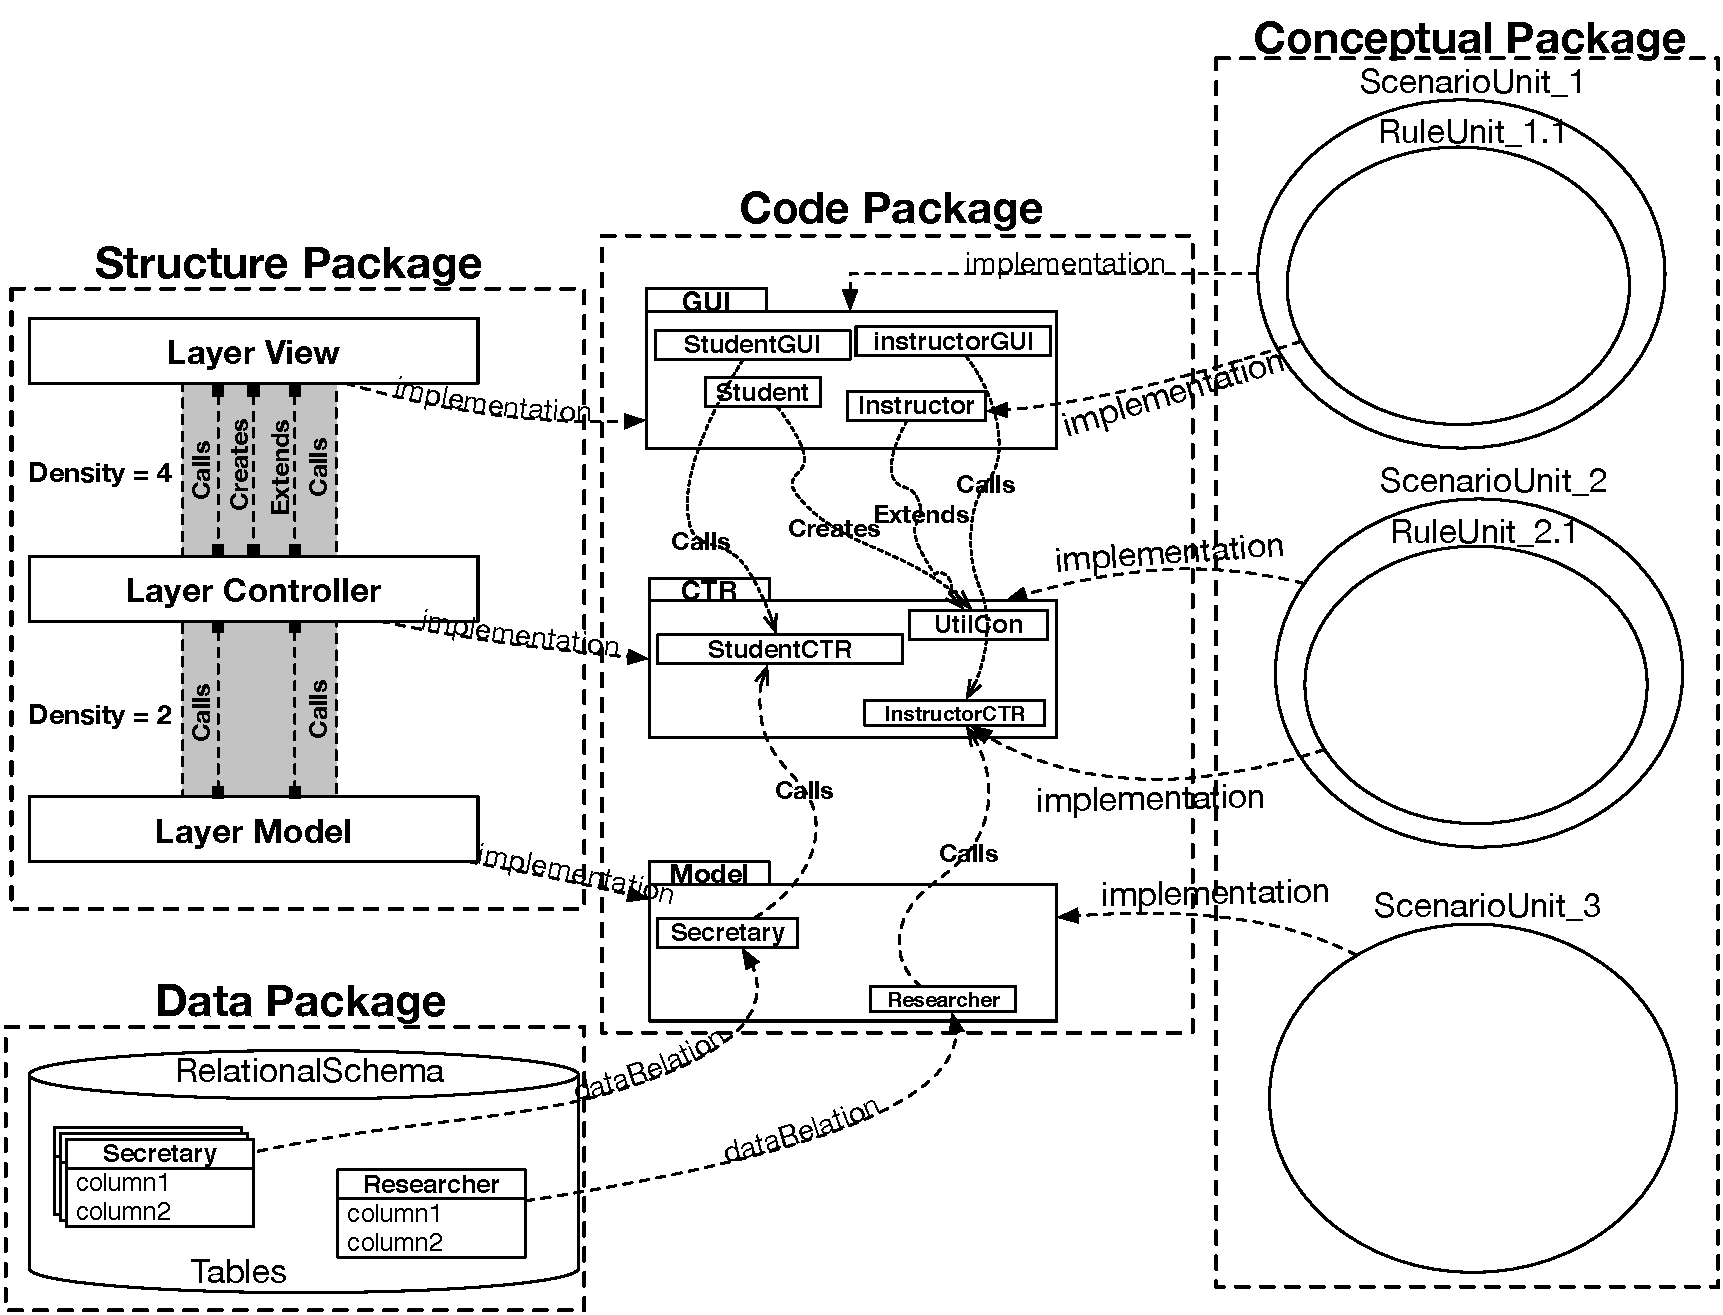
\includegraphics[scale=0.58]{figuras/NewSystemVersion}
	\caption{Motivation and running example.}
	\label{fig:system}
\end{figure*}

This section introduces an illustrative and motivating scenario that will be used as running example along each phase of the approach presented in this paper, and that will be detailed in Section~\ref{sec:the_approach}. As a demonstration of the problem of propagation of changes in KDM levels/packages, let us consider a toy system that is based on a well know Model View Controller (MVC) design pattern. As noted in Figure~\ref{fig:system} this system is split in four KDM levels/packages, which are illustrated in the figure bounded by dashed lines shape. Following is described each KDM levels/packages and its meaning regarding to the illustrated system.

\begin{itemize}

\item Code Package - represents the source-code (physical artifacts). In Figure~\ref{fig:system} is is possible to see three packages: (\textit{i}) \texttt{GUI}, (\textit{ii}) \texttt{CTR}, and (\textit{iii} \texttt{Model}). The first one, \texttt{GUI}, contains four classes, \texttt{StudentGUI}, \texttt{InstructorGUI}, \texttt{Student}, and \texttt{Instructor}. The second package contains three classes: \texttt{StudentCTR}, \texttt{UtilCon}, \texttt{InstructorCTR}. Then, the third one owns two classes, \texttt{Secretary} and \texttt{Researcher}. Note that these classes are related to each other by means of primitive relationships, such as: \texttt{Calls}, \texttt{Creates}, \texttt{Extends}, etc;

\item Structure Package - illustrates the system's architecture, herein the system is based on MVC. As noted in Figure~\ref{fig:system} each rectangle depicts a layer, i.e., \texttt{View}, \texttt{Controller}, and \texttt{Model}. For the first layer, we have associated \texttt{View} with the package \texttt{GUI}. In KDM this kind of association is done by means of the meta-attribute \texttt{implementation}, which are depicted by the dashed arrows. Similarly, \texttt{Controller} was associated with the package \texttt{CTR}, and the layer \texttt{Model} was associated with the package \texttt{Model}, respectively. Regarding to the relationships among the layers, it is possible to visualize pipes between two layers (see Figure~\ref{fig:system}. These pipes represents the corresponding aggregated relationship, which represents the number summing all primitive relationships among layers. For instance, the aggregation relationship between the layer \texttt{View} and the layer \texttt{Controller} are represented by the relationships: \texttt{Calls}, \texttt{Creates}, \texttt{Extends}, and another \texttt{Calls} from the Code Package. Summing up these relationships the density value is 4. Following the same idea the relationship between the layer \texttt{Controller} and layer \texttt{Model} is 2;  
  
\item Conceptual Package - illustrates the system's business rules domain. Note that this system owns three scenarios, each of them are associated with a package from Code Package by means of the association \texttt{implementation}, see the dashed arrows. Further, each scenario contains a rule except the last one. In it turn, each rule is associated with a class from Code package, again using the association \texttt{implementation};

\item Data Package - depicts the system's database and its tables. Herein, it is possible to notice that the depicted system owns a set of Plain Old Java Objects (POJOS), they are: Student, Instructor, Secretary, and Researcher. All of these POJOS are also Object Relational Mapping (ORM), i.e., they are mapped to the Data package using the metaclasse RelationalTable. 

\end{itemize}

%(\textit{i}) Code Package, which represents the source-code (physical artefacts), (\textit{ii}) Structure Package, that illustrates the system's architecture, herein the system is based on MVC, (\textit{iii}) Data Package, which depicts the system's database and its tables, and (\textit{iv}) Conceptual Package, which is intended to be the basis for formal and detailed natural language declarative description of a complex entity, such as a business


%owns three layers, they are: (\textit{i}) ``View'', (\textit{ii}) ``Controller'', and (\textit{iii}) ``Model''. Inside of each layer there is at least one package. For instance, the relationships ``GUI inside View'', ``CTR inside Controller'', and ``model inside Model'' mean that ``GUI'', ``CTR'' and ``model'' are contained in ``View'', ``Controller'' and ``Model'', respectively or in some sub-container of  them, transitively. Similarly, the relationship ``StudentGUI inside GUI'' means that ``StudentGUI'' is in container ``GUI'' or in some sub-container of ``GUI''.



%Furthermore, it is possible to notice that the depicted system owns a set of Plain Old Java Objects (POJOS), they are: ``Student'', ``Instructor'', ``Secretary'', and ``Researcher''. All of these POJOS are also Object Relational Mapping (ORM).

Considering this system it is possible to highlight some problem or even to add new requirements. For instance, a problem that can be noticed is that both classes \texttt{Student} and \texttt{Instructor} should be contained in \texttt{Model} package not in \texttt{GUI} package, respectively. In order to fix this problem, one should apply a refactoring - for instance, \textit{Move Class}.
%

%

Regarding to a new requirement let's pretend someone has identified that the class \texttt{Student} is doing work that should be done by two classes - it contains attributes to hold informations upon student's addresses. In order to fulfill this new requirement one should apply the refactoring \textit{Extract Class} and creates a new class named Address (which is a POJO and also an ORM) and move all student's attributes related to address to this new class.

%The action of this refactoring should propagate throughout other KDM's levels, such as the data level\footnote{The KDM's level that contains information on data base schema, table, column, primary key, etc}. 

However, in both described refactoring it is necessary a skilled domain expert into KDM to identify all the metaclasses in the system which involve/reference the classes aforementioned and correct them respectively in all KDM packages, i.e., propagate all refactoring's impact throughout all KDM's packages. 

For instance, considering the refactoring \textit{Move Class} (move \texttt{Student} and \texttt{Instructor} from \texttt{GUI} package to \texttt{Model} package) changes should be propagated to the Structure Package and to the Conceptual Package to maintain the model synchronized. For instance, the \texttt{density}, i.e., aggregation relation ship between the layer \texttt{View} and the layer \texttt{Controller} would change from 4 to 2 - once the primitives relationships \texttt{Create} and \texttt{Extends} would no longer exist from the package \texttt{GUI} to the package \texttt{CTR}. On the other hand, the resulting of this refactoring would update the density between the layer \texttt{Model} and \texttt{Controller}, instead of 2 it should be 4, as \texttt{Creates} and \texttt{Extends} were also moved along with its classes, \texttt{Student} and \texttt{Instructor}. Concerning to the Conceptual package, the  RuleUnit\_1.1 that is associated with \texttt{Student} should also be moved to ScenarioUnit\_3. 

Regarding to the refactoring \textit{Extract Class}, the extracted class \texttt{Address} would be a POJO (it would be contained in Model package) and it would also be an ORM - therefore, the action of this refactoring should be propagated throughout  the Data package, i.e., the instance of \texttt{Address} should be associated with a metaclass \texttt{RelationalTable}, and its attributes should be associated with  of \texttt{ColumnSet}.

%, i.e., the relationship among the layers should be propagated automatically. Similarly, considering the refactoring \textit{Extract Class}, where a new POJO and ORM class is created, the data's level also should be propagated.

These propagation seen to be easy to apply, however, in a complex system comprising all kdm's packages/levels, propagate all changes after a refactoring is a difficult and error-prone task. Even identifying the affected parts of the KDM's packages/levels is not an easy and straightforward process. In order to fulfill this limitation and create an automatized process we have devised Propagation-Aware Refactorings (PARef) that contains three main steps. The first step is the identification of all dependent elements related to a specific refactoring. In the second step the refactoring of all identified elements are performed using a model-to-model transformation language - the third step is the propagation of changes in order to keep all the dependent models synchronized. %In the following sections we show in detail that change propagation in KDM is a complex process that can be solved semi-automatically and, hence, efficiently and precisely if we provide a rigorous theoretical background. 
In the following sections we show the theoretical background need to fully understand our approach. Then, our approach is presented in Section~\ref{sec:the_approach}.


%  one should identify and change all the relationship after the refactoring

%Let us consider a new user requirement that the both classes ``Student'' and ``Instructor'' should not longer be represented in the layer ``View''. Instead, these classes should be allocated into a new layer, e.g., layer ``Model''. This new requirement would require the application of a refactoring - for instance, \emph{Extract Package}. However, such a situation would require a skilled domain expert into KDM to identify all the metaclasses in the system which involve/reference the classes aforementioned and correct them respectively in all KDM levels. Apparently, in a complex system comprising all kdm's levels, this is a difficult and error-prone task. Even identifying the affected parts of the KDM's levels is not an easy and straightforward process. 

%Our approach contains three main steps. The first one is the identification of all dependent elements. In the second step the refactoring of all identified elements are performed and the third one is the propagation of changes in order to keep all the dependent models synchronised. In the following sections we show in detail that change propagation in KDM is a complex process that can be solved semi-automatically and, hence, efficiently and precisely if we provide a rigorous theoretical background. 
 